%%%%%%%%%%%%%%%%%%%%%%%%%%%%%%%%%%%%%%%%%
% baposter Landscape Poster
% LaTeX Template
% Version 1.0 (11/06/13)
%
% baposter Class Created by:
% Brian Amberg (baposter@brian-amberg.de)
%
%
% License:
% CC BY-NC-SA 3.0 (http://creativecommons.org/licenses/by-nc-sa/3.0/)
%
%%%%%%%%%%%%%%%%%%%%%%%%%%%%%%%%%%%%%%%%%

%----------------------------------------------------------------------------------------
%PACKAGES AND OTHER DOCUMENT CONFIGURATIONS
%----------------------------------------------------------------------------------------

\documentclass[landscape,a1paper,fontscale=0.5]{baposter} % Adjust the font scale/size here

\usepackage{graphicx} % Required for including images
\graphicspath{{figures/}} % Directory in which figures are stored

\usepackage{amsmath} % For typesetting math
\usepackage{amssymb} % Adds new symbols to be used in math mode

\usepackage{booktabs} % Top and bottom rules for tables
\usepackage{enumitem} % Used to reduce itemize/enumerate spacing
\usepackage[font=small,labelfont=bf]{caption} % Required for specifying captions to tables and figures
\usepackage{tcolorbox}
\usepackage{listings}
\usepackage{xcolor}
\usepackage{multicol} % Required for multiple columns
\setlength{\columnsep}{1.5em} % Slightly increase the space between columns
\setlength{\columnseprule}{0mm} % No horizontal rule between columns
\usepackage[T1]{fontenc}
\usepackage{tikz} % Required for flow chart
\usetikzlibrary{shapes,arrows} % Tikz libraries required for the flow chart in the template
\usepackage{fix-cm}
\newcommand{\compresslist}{ % Define a command to reduce spacing within itemize/enumerate environments, this is used right after \begin{itemize} or \begin{enumerate}
\setlength{\itemsep}{1pt}
\setlength{\parskip}{0pt}
\setlength{\parsep}{0pt}
}

\definecolor{lightblue}{rgb}{.54,.824,1.} % Defines the color used for content box headers
\definecolor{whiteblue}{RGB}{240,255,255} % Defines the color used for content box headers

\newcommand{\reducedstrut}{\vrule width 0pt height .9\ht\strutbox depth .9\dp\strutbox\relax}
\newcommand{\cmt}[1]{%
  \begingroup
  \setlength{\fboxsep}{0pt}% 
  \color{white}
  \textnormal{
  \colorbox{blue}{\reducedstrut#1\/}}%
  \endgroup
}

\begin{document}

\begin{poster}
{
headershade=plain,
headerborder=closed, % Adds a border around the header of content boxes
colspacing=1em, % Column spacing
bgColorOne=white, % Background color for the gradient on the left side of the poster
bgColorTwo=white, % Background color for the gradient on the right side of the poster
borderColor=lightblue, % Border color
headerColorOne=blue, % Background color for the header in the content boxes (left side)
headerColorTwo=blue, % Background color for the header in the content boxes (right side)
headerFontColor=white, % Text color for the header text in the content boxes
boxColorOne=lightblue, % Background color of the content boxes
textborder=rounded, % Format of the border around content boxes, can be: none, bars, coils, triangles, rectangle, rounded, roundedsmall, roundedright or faded
eyecatcher=true, % Set to false for ignoring the left logo in the title and move the title left
headerheight=0.\textheight, % Height of the header
headershape=rounded, % Specify the rounded corner in the content box headers, can be: rectangle, small-rounded, roundedright, roundedleft or rounded
headerfont=\Large\bf\textsf, % Large, bold and sans serif font in the headers of content boxes
%textfont={\setlength{\parindent}{1.5em}}, % Uncomment for paragraph indentation
linewidth=2pt, % Width of the border lines around content boxes
columns=3
}
%----------------------------------------------------------------------------------------
%TITLE SECTION 
%----------------------------------------------------------------------------------------
%
{} % First university/lab logo on the left
{} % Poster title
{} % Author names and institution
{} % Second university/lab logo on the right

%----------------------------------------------------------------------------------------
%RooFit, RooStats and HistFactory
%----------------------------------------------------------------------------------------
\sffamily
\headerbox{}{name=intro,column=0,row=0,headerborder=none,textborder=none,headerColorOne=white,headershade=plain,boxColorOne=white}{
\begin{center}{\textcolor{lightblue}{\textbf{\fontsize{25}{25}\selectfont RooFit, RooStats \& HistFactory}}}

{\Large a python data science{\it Cheat Sheet}}\end{center}
%\vspace{0.5em} % When there are two boxes, some whitespace may need to be added if the one on the right has more content
}

%----------------------------------------------------------------------------------------
%CONTACT INFORMATION
%----------------------------------------------------------------------------------------

\headerbox{Contact Information}{name=contact,column=2,above=bottom}{ % This block is as tall as the references block

\begin{description}\compresslist
\item[Web] www.university.edu/smithlab
\item[Email] john@smith.com
\item[Phone] +1 (000) 111 1111
\end{description}
}

%----------------------------------------------------------------------------------------
%About RooFit
%----------------------------------------------------------------------------------------

\headerbox{A Simple Example}{name=simple,column=0,below=intro}{ % This block's bottom aligns with the bottom of the conclusion block
\begin{tcolorbox}[colback=blue!5!white,colframe=blue!75!black]
\tt{
import ROOT\\
w = ROOT.RooWorkspace()\\
w.factory(`Gaussian::g(x[-5,5],mu[-3,3],sigma[1])')\\
w.factory(`Exponential::e(x,tau[-.5,-3,0])')\\
w.factory(`SUM::model(s[50,0,100]*g,b[100,0,1000]*e)')\\
x = w.var(`x')\\
pdf = w.pdf(`model')\\
frame = x.frame()\\
data = pdf.generate(ROOT.RooArgSet(x))\\
data.plotOn(frame)\\
fitResult = pdf.fitTo(data,ROOT.RooFit.Save())\\
pdf.plotOn(frame)\\
frame.Draw()}
\begin{center}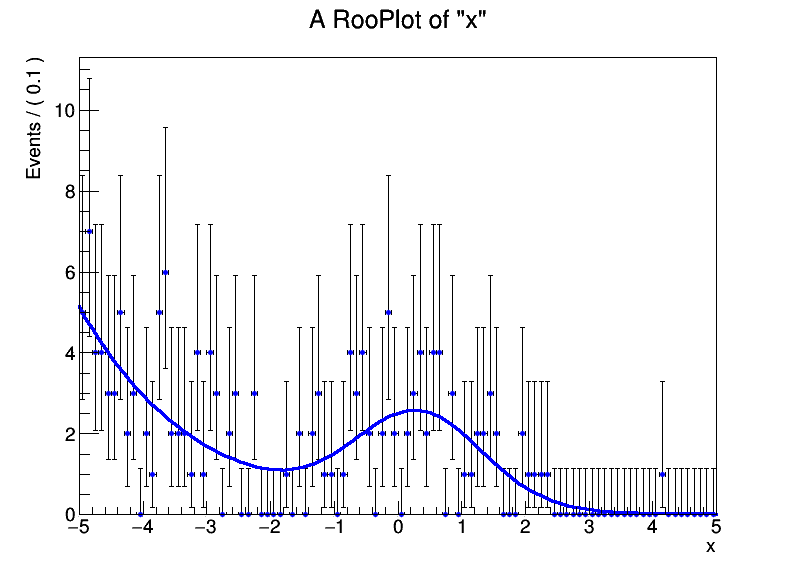
\includegraphics[width=0.55\linewidth]{simpleexample01}\end{center}
\end{tcolorbox}

}


%----------------------------------------------------------------------------------------
%RooStats
%----------------------------------------------------------------------------------------

\headerbox{Statistical Tests with RooStats}{name=tests,column=2,span=1,row=0}{
\begin{tcolorbox}[colback=blue!5!white,colframe=blue!75!black,width=\linewidth,title=Profile Likelihood]
\tt{
pl = ROOT.RooStats.ProfileLikelihoodCalculator(data,ModelConfig)\\
pl.SetConfidenceLevel(0.683) \hfill \cmt{set desired interval}\\
interval = pl.GetInterval() \hfill\cmt{perform calculation}\\
firstPOI = mc.GetParametersOfInterest().first() \hfill\cmt{only one POI}\\
lowerLimit = interval.LowerLimit(firstPOI)\hfill\cmt{extract limits}\\
upperLimit = interval.UpperLimit(firstPOI)\hfill\cmt{this is a number}\\
plot = ROOT.RooStats.LikelihoodIntervalPlot(interval) \\
plot.Draw() \hfill\cmt{Custom plot object but regular frame->plotOn also works.}
\begin{center}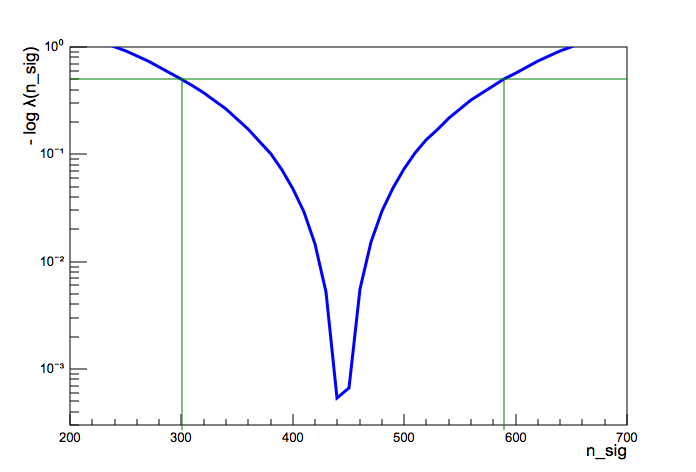
\includegraphics[width=0.5\linewidth]{pl}\end{center}
}
\end{tcolorbox}

\begin{tcolorbox}[colback=blue!5!white,colframe=blue!75!black,width=\linewidth,title=Hypothesis Test (asymptotic formula)]
\tt{
ac = ROOT.RooStats.AsymptoticCalculator(data, sbModel, bModel)\\
asResult = ac.GetHypoTest() \hfill\cmt{where \tt{sbModel} is signal+background}\\
asResult.Print() \hfill\cmt{\tt{bModel} = background only. Gives p-value \& $Z_0$}
}
\end{tcolorbox}


\begin{tcolorbox}[colback=blue!5!white,colframe=blue!75!black,width=\linewidth,title=Limits using Hypothesis Test Inversion (CLs Limits)]
\tt{
ac = ROOT.RooStats.AsymptoticCalculator(data, sbModel, bModel)\\
calc = ROOT.RooStats.HypoTestInverter(ac) \hfill\cmt{as above}\\
calc.SetConfidenceLevel(0.95) \hfill\cmt{desired limit}\\
calc.UseCLs(True)\hfill\cmt{scan CLs+b or CLs values}\\
toymcs = calc.GetHypoTestCalculator().GetTestStatSampler()\\
profll = ROOT.RooStats.ProfileLikelihoodTestStat(sbModel.GetPdf())\\
toymcs.SetTestStatistic(profll)\hfill\cmt{Profile likelihood test statistics}\\
calc.SetFixedScan(npoints,poi.getMin(),poi.getMax())\hfill\cmt{set range}\\
r = calc.GetInterval()\hfill\cmt{or scan until reaching the desired precision}\\
upperLimit = r.UpperLimit()\hfill\cmt{the result for this confidence level.}\\
plot = ROOT.RooStats.HypoTestInverterPlot("HTI\_Result\_Plot",\\
\hspace*{7cm}"HypoTest Scan Result",r)\\
plot.Draw("CLb 2CL")
}
\begin{center}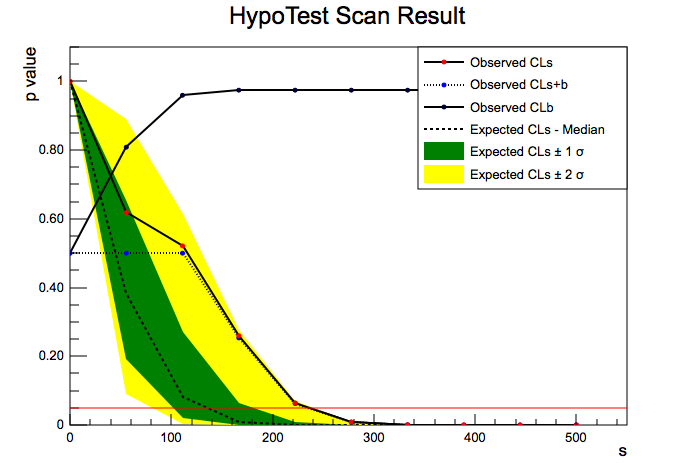
\includegraphics[width=0.5\linewidth]{cls}\end{center}

\end{tcolorbox}

}
%----------------------------------------------------------------------------------------
%Workspaces
%----------------------------------------------------------------------------------------



\headerbox{Workspaces and Histfactory}{name=workspaces,column=0,span=2,below=simple,bottomaligned=tests}{ % This block's bottom aligns with the bottom of the conclusion block
\begin{multicols}{2}
\begin{tcolorbox}
[colback=blue!5!white,colframe=blue!75!black,width=\linewidth]
\tt{
w = ROOT.RooWorkspace("w")\hfill \cmt{Make a workspace}\\
getattr(w,`import')(pdf1)\hfill \cmt{Move a pdf into the workspace}\\
w.factory(`SUM::model(n\_sig[5,0,10]*pdf1,n\_bkg[10,0,100]*pdf2)')\\
w.var("n\_sig").setVal(2)\hfill \cmt{Factory can be used to create models}\\
model = w.pdf("model")\hfill \cmt{objects (e.g PDFs) are extracted by name}\\
data = model.generate(ROOT.RooArgSet(x))\hfill \cmt{data to be used}\\
getattr(w,`import')(data)\hfill \cmt{most WS's need a PDF and data}\\
mc = ROOT.RooStats.ModelConfig("ModelConfig",w)\hfill \cmt{configure model}\\
mc.SetPdf(model)\hfill \cmt{target subset of variables}\\
mc.SetParametersOfInterest(ROOT.RooArgSet(w.var("n\_sig")))\hfill \cmt{POI}\\
mc.SetSnapshot(ROOT.RooArgSet(w.var("n\_sig")))\hfill \cmt{preserve values}\\
mc.SetObservables(ROOT.RooArgSet(w.var("x")))\hfill \cmt{target range}\\
w.defineSet("nuisParams","n\_bkg")\hfill \cmt{there can be hundreds of NPs}\\
nuis = getattr(w,`set')("nuisParams")\hfill \cmt{added to WS as normal}\\
mc.SetNuisanceParameters(nuis) \hfill \cmt{NPs distingushed from POIs in model}\\
getattr(w,`import')(mc)\hfill \cmt{import ModelConfig to WS}\\
w.writeToFile("outputdir/name.root",True)\hfill \cmt{save the workspace to file}
}
\end{tcolorbox}
\begin{tcolorbox}
[colback=blue!5!white,colframe=blue!75!black,width=\linewidth]
\tt{
meas = ROOT.RooStats.HistFactory.Measurement("meas", "meas")\\
meas.SetPOI( "SigXsecOverSM" )\\
chan = ROOT.RooStats.HistFactory.Channel( "SignalRegion" )\\
chan.SetStatErrorConfig(0.05, "Poisson")\\
chan.SetData( data\_hist )\\
signal = ROOT.RooStats.HistFactory.Sample( "signal" )\\
signal.SetHisto( signal\_hist )\\
signal.AddNormFactor( "SigXsecOverSM", 1, 0, 3)\\
signal.AddOverallSys( "flat\_uncertainty",  low\_val, high\_val )\\
signal\_shape = ROOT.RooStats.HistFactory.HistoSys("shape\_uncert")\\
signal\_shape.SetHistoHigh( sig\_up\_hist )\\
signal\_shape.SetHistoLow( sig\_down\_hist )\\
signal.AddHistoSys( signal\_shape )\\
chan.AddSample( signal )\\
hist2workspace =\\
\hspace*{1.5cm}ROOT.RooStats.HistFactory.HistoToWorkspaceFactoryFast(meas)\\
workspace = hist2workspace.MakeSingleChannelModel(meas, chan)
}
\end{tcolorbox}
\end{multicols}
}


%----------------------------------------------------------------------------------------
%Fitting
%----------------------------------------------------------------------------------------

\headerbox{Models and Fitting}{name=fitting,column=1}{ % This block's bottom aligns with the bottom of the conclusion block
For a set of PDFs e.g. \tt{signalpdf} and \tt{backgroundpdf} and a fractional normalization \tt{fsig}:
\begin{tcolorbox}
[colback=blue!5!white,colframe=blue!75!black,width=\linewidth]
\tt{
fsig = ROOT.RooRealVar("fsig","signal fraction",0.5,0.,1.)\\
model = ROOT.RooAddPdf("model","model",\\
\hspace*{1.8cm}RooArgList(signalpdf,backgroundpdf),RooArgList(fsig))
}
\end{tcolorbox}

We can create a negative log-likelihood (nll) function and from this and profile log-likelohood (pll) function. These relate estimators for the parameters in a model to some data.

\begin{tcolorbox}
[colback=blue!5!white,colframe=blue!75!black,width=\linewidth]
\tt{
nll = pdf.createNLL(data)\\
pll = nll.createProfile(paramOfInterest)
}
\end{tcolorbox}
Various minimizers are available through the minuit package, these can act on all parameters or just those specified.
\begin{tcolorbox}
[colback=blue!5!white,colframe=blue!75!black,width=\linewidth]
\tt{
m  = ROOT.RooMinimizer(nll)\\
m.migrad() \hfill\cmt{efficient and fast, struggles with nonlinearities}\\
m.hesse()\hfill\cmt{calculates the full error matrix from second derivatives}\\
m.minos(ParametersOfInterest)\hfill\cmt{correct even if non-parabolic, but slow}
}
\end{tcolorbox}

}


%----------------------------------------------------------------------------------------
%RooFit Data types
%----------------------------------------------------------------------------------------

\headerbox{RooVariables, RooPdfs, and Data}{name=vars,column=0,span=3,below=workspaces,above=bottom}{ % This block's bottom aligns with the bottom of the conclusion block

\begin{multicols}{3}
\begin{tcolorbox}[colback=blue!5!white,colframe=blue!75!black,width=1.\linewidth,title=Variables and P.D.Fs]
\tt{
observable = ROOT.RooRealVar("x","x",-10,10)\\
mean = ROOT.RooRealVar("mean","Mean",-10,10)\\
sigma = ROOT.RooRealVar("sigma","Width",3,-10,10)\\
gauss = ROOT.RooGaussian("gauss","pdf title",x,mean,sigma)
}
\end{tcolorbox}

\columnbreak

\begin{tcolorbox}[width=2\linewidth,colback=blue!5!white,colframe=blue!75!black,title=Common P.D.Fs]
\begin{tabular}{l | l c}
\tt{ROOT.RooBifurGauss("name", "title", $x$, $\mu$, $\sigma_L$, $\sigma_R$)} & Bifurcated Gaussian & $f(x;\mu,\sigma)=\frac{1}{N}\cdot \exp(-(x-\mu)^2/(2\sigma(x-\mu)^2)$\\
\tt{ROOT.RooExponential("name", "title", $x$, $c$)} & Exponential & $f(x;c)=\frac{1}{N}\exp (c x)$\\
\tt{ROOT.RooPolynomial("name", "title", $x$, RooArgList($c_1$,$c_2$)} & Polynomial & $f(x;c_0,...,c_n)=\frac{1}{N}\cdot\left(1+\sum_{k=1}^{n}c_kx^k\right)$\\
\tt{ROOT.RooPoisson("name", "title", $x$, $\eta$)} & Poisson & $f(x;\eta)=\frac{1}{x!}\cdot\eta^x\exp(-\eta)$
\end{tabular}
\end{tcolorbox}

\columnbreak
\vspace*{2.2cm}
\begin{flushright}

\includegraphics[width=0.25\linewidth]{dianahep} 

\includegraphics[width=0.25\linewidth]{root}
\end{flushright}
\columnbreak


\end{multicols}
}

%----------------------------------------------------------------------------------------
%Working with data
%----------------------------------------------------------------------------------------



\headerbox{Using Data}{name=data,column=1,below=fitting,above=workspaces}{ % This block's bottom aligns with the bottom of the conclusion block
Data can be imported from histograms or generated from a model.
\begin{tcolorbox}[colback=blue!5!white,colframe=blue!75!black,width=\linewidth]
\tt{
hh = ROOT.TH1F("hh","some histogram",21,-10,10)\\
x = ROOT.RooRealVar("x","x",-10,10)\\
real\_data = ROOT.RooDataHist("data","dataset with x",x,hh)\\
pseudo\_data = model.generate(ROOT.RooArgSet(x),10000)
}
\end{tcolorbox}

}


%----------------------------------------------------------------------------------------

\end{poster}

\end{document}
